% for sublime text 3
%!TEX root = diss.tex

\chapter{Related Work}
\label{ch:rel-work}
 
The task of coherence modeling has received a lot of attention due to its key impact in other natural language processing systems. 
In this thesis, we propose a novel approach to local coherence modeling based on graph representations of texts. 
We apply our approach to two types of graphs.  
The first type captures coreferent relations between named entity mentions in a text.
The second one represents lexical relations among words in a text.  
Our coherence model is evaluated with respect to its impact on readability assessment and text summarization. 

Accordingly, we first review entity-based approaches to local coherence (Section \ref{sec:rel-entity-models}). 
We then survey lexical approaches (Section \ref{sec:rel-ent-grid}). 
Finally, we discuss applications of local coherence model that have been introduced in the literature, particularly readability assessment and summarization tasks (Section \ref{sec:rel-coh-applications}). 
% A coherent text consists of a sequence of topics in a structured way \cite{marcu97b,hearst97,gallery03}. 
% Related models are often constructed as sequential topical models. 
% Topics are modeled by a language model \cite{blei01} or Bayesian topic models \cite{eisenstein08}.
% For modeling the temporal structure, early research uses a Hidden Markov Model \cite{barzilay04}, and  
% later research employs sequential neural networks \cite{}. 

\section{Entity-based Approaches to Local Coherence}
\label{sec:rel-entity-models}

The primary steps of the research presented in this thesis are inspired by entity-based coherence models. 
In this section, we explain details of two popular entity-based models: the entity grid model, and the entity graph model. 
We also briefly discuss their extensions.  

\paragraph{Historical Review.} Entity-based approaches to local coherence have a long history within the linguistic literature \cite{kuno72,halliday76,prince81a,joshi98}.
Most approaches are common in the primary assumption that coherence is perceived with respect to how entities are introduced and discussed in a text. 
Texts that keep referring to similar entities are supposed to be more coherent than those with random and unexpected switches from one entity to another. 
This premise is supported by different theories, one of which is the centering theory \cite{grosz95,joshi98} that is discussed in Chapter \ref{ch:coh-models}. 

A great deal of research has been devoted to directly implement the centering theory \cite{miltsakaki00,karamanis04a}. 
This is challenging because a computational model needs to determine how to instantiate parameters of the theory that are often underspecified. 
Interestingly, \newcite{poesio04b} note that even for basic parameters of Centering Theory such as ``utterance'', ``realization'', and ``ranking'', multiple interpretations have been developed, because in the original theory of centering these concepts are not explicitly specified. 
As an instance, in some papers entities are ranked with respect to the grammatical function \cite{brennan87,grosz95} of entity occurrences in a text, and in some other papers those are ranked with respect to the position of entity mentions in sentences \cite{prince81a}, the familiarity status or the thematic role \cite{strube.cl99,moens08}.
As a result, two instantiations of the same theory make different predictions for the same input.  

Some studies try to avoid this by finding an instantiation of parameters which is most consistent with observable data \cite{strube.cl99,karamanis04a,poesio04b}. 
Some others adopt a specific instantiation so that the performance of the coherence model improves for a specific task. 
For example, \newcite{miltsakaki00} annotate a corpus of student essays with entity transition information, and then show that the distribution of transitions correlates with human grades. 
Analogously, \newcite{hasler03} investigate whether the centering theory can be used in evaluating the readability of text by annotating summaries produced by humans or machines with the entity transition information. 
To sum up, \newcite{poesio04b} demonstrate that the predictive power of the models that directly implement centering theory is highly sensitive to their parameter instantiations.  

\newcite{barzilay05a,barzilay08} propose a general framework for coherence modeling.  
The main goal of this framework is to eliminate the need to human annotations for parameters in the centering theory, regardless of what the evaluation task is. 
By some inspirations from the theory, this model hypothesizes that the distribution of entities in coherent texts reveal certain regularities that make these texts recognizable from incoherent ones. 
These regularities can be learned by machine learning approaches.  
Since this model has been the core of many research in the area of coherence modeling (including the research presented in this thesis), we explain details of this model.    

\subsection{The Entity Grid Model}
\label{sec:rel-ent-grid} 

\newcite{barzilay05a,barzilay08} are the first who proposed a general  computational approach to local coherence modeling based on the entity relations across adjacent sentences.  
Supported by some linguistic work such as the centering theory \cite{grosz95} and other entity-based theories of discourse \cite{prince81a}, they assume that the distribution of entities in coherent texts exhibits certain regularities that can be reflected in a grid topology, which is called the entity grid. 
In this thesis we refer to this model as the entity grid model because its key idea is to represent the distribution of entities (see Chapter \ref{ch:coherence} for the definition of entities) across sentences in a text by a grid.   
In practice, mentions of an entity are linked together in order to show that they are referring to the same entity. 
Connections between mentions not only show that those are referring to the same entity but also indicate that sentences that contain those mentions are (almost) about the same topic or information \cite{barzilay08}. 

\subsubsection{Text Representation: Entity Grid}

In this model each text is represented by a grid, which is a two dimensional array whose rows correspond to entities, and columns are matching to sentences.
An entry $r_{i;j}$ in a grid describes the syntactic role of entity $i$ in sentence $j$ if the entity is mentioned in the sentence. 
The syntactic roles are categorized as subject (S), object (O), or all other syntactic roles (X). 
In addition, if an entity is not mentioned in a sentence, a special marker (-) fills the corresponding entry $r_{i;j}$. 
Finally, if a sentence contains several mentions of one entity, their corresponding entry describes the most important grammatical role of the mentions: subject if possible, then object, or finally other. 

The discussion of the grid develops around the important question of which textual units are to be considered mentions of an entities, and how different mentions are to be linked to represent an entity. 
A perfect solution in this regard would use a coreference resolution system to recognize mentions, i.e.\ noun phrases, and to link arbitrary mentions to the same entities and discarding noun phrases which do not correspond to an entity. 
Since coreference resolution systems are far from prefect\footnote{The highest reported precision of a coreference system on the ? dataset is ?.}, and tend to work even more poorly on incoherent texts, this approach is not generally one utilized.  
Moreover, a non-perfect general coreference system introduces more noise to a coherence model than what it fixes \cite{barzilay08}.  
As an alternative, implementations of the entity grid model tend to employ all noun phrases as mentions and perform a heuristic, but strict and simple, coreference resolution. 
These models connect all mentions that have an identical head noun as one entity. 
Detailed discussions of this heuristic are given in \newcite{poesio04c} and \newcite{elsner10}. 

As an example consider the sample text\footnote{The text with ID D31010, taken from Document Understanding Conference (DUC-?) dataset, which we use in one of our experiments. Numbers are not marked because they are filtered out in preprocessing.} in Example \ref{ex:rel-text}. 
In this example, noun phrases are marked with brackets as an indication of mentions. 
Mentions in a sentence are associated with their syntactic functions in the sentence, noted with a letter (S: subject, O: object, and X: others) next to the brackets. 
%/hits/fast/nlp/mesgarmn/Data/ACL13/SummaryCoherence/texts/
%D31010.M.100.T.E.txt. Nubembers (e.g. 29) are filtered out in preprocessing.}  

\begin{examples}
\label{ex:rel-text}
\begin{tabular}{l@{\space}p{12.5cm}}
 $s_0$: &[An arctic cold wave]\textbf{\textsubscript{S}}, [the worst]\textbf{\textsubscript{X}} in [10 years]\textbf{\textsubscript{X}}, hit [parts]\textbf{\textsubscript{O}} of [Europe]\textbf{\textsubscript{X}}, bringing [sub-zero temperatures]\textbf{\textsubscript{O}} and killing [scores]\textbf{\textsubscript{O}} of [people]\textbf{\textsubscript{X}}. \\

 $s_1$: & Hardest hit were [Poland]\textbf{\textsubscript{S}}, [Bulgaria]\textbf{\textsubscript{S}}, and [Romania]\textbf{\textsubscript{S}} as well as [parts]\textbf{\textsubscript{S}} of [central]\textbf{\textsubscript{X}} and [eastern France]\textbf{\textsubscript{X}}. \\

$s_2$: &In [Poland]\textbf{\textsubscript{X}}, [three weeks]\textbf{\textsubscript{X}} of [sub-zero temperatures]\textbf{\textsubscript{X}} killed [at least 85 people]\textbf{\textsubscript{O}} in [November]\textbf{\textsubscript{X}}, 29 more than in [all]\textbf{\textsubscript{X}} of [the previous winter]\textbf{\textsubscript{S}}. \\


$s_3$: &[Most]\textbf{\textsubscript{S}} of [the victims]\textbf{\textsubscript{X}} were homeless [whose deaths]\textbf{\textsubscript{X}} by [exposure]\textbf{\textsubscript{X}} were alcohol related. \\

$s_4$: &[Blizzards]\textbf{\textsubscript{X}} and [cold temperatures]\textbf{\textsubscript{S}} also hit [Bulgaria]\textbf{\textsubscript{X}} and [Romania]\textbf{\textsubscript{O}}, stranding [hundreds]\textbf{\textsubscript{O}} in [their cars]\textbf{\textsubscript{X}}. \\

$s_5$: &Elsewhere, [snow]\textbf{\textsubscript{S}} blanketed [the Italian island]\textbf{\textsubscript{O}} of [Capri]\textbf{\textsubscript{X}} for [the first time]\textbf{\textsubscript{X}} in [10 years]\textbf{\textsubscript{X}}. 
\end{tabular}
\end{examples}
%%(ROOT (S (NP (NP (DT An) (JJ arctic) (JJ cold) (NN wave)) (, ,) (NP (NP (DT the) (JJS worst)) (PP (IN in) (NP (CD 10) (NNS years)))) (, ,)) (VP (VBD hit) (NP (NP (NNS parts)) (PP (IN of) (NP (NNP Europe)))) (, ,) (S (VP (VP (VBG bringing) (NP (JJ sub-zero) (NNS temperatures))) (CC and) (VP (VBG killing) (NP (NP (NNS scores)) (PP (IN of) (NP (NNS people)))))))) (. .)))

%%(ROOT (S (S (VP (ADVP (RBS Hardest)) (VBN hit))) (VP (VBD were) (NP (NP (NP (NNP Poland)) (, ,) (NP (NNP Bulgaria)) (, ,) (CC and) (NP (NNP Romania))) (CONJP (RB as) (RB well) (IN as)) (NP (NP (NNS parts)) (PP (IN of) (NP (NP (JJ central)) (CC and) (NP (JJ eastern) (NNP France))))))) (. .)))

%%(ROOT (S (PP (IN In) (NP (NNP Poland))) (, ,) (NP (NP (CD three) (NNS weeks)) (PP (IN of) (NP (JJ sub-zero) (NNS temperatures)))) (VP (VBD killed) (NP (QP (IN at) (JJS least) (CD 85)) (NNS people)) (PP (IN in) (NP (NNP November))) (, ,) (PP (ADVP (NP (CD 29)) (RBR more)) (IN than) (IN in) (NP (NP (DT all)) (PP (IN of) (NP (DT the) (JJ previous) (NN winter)))))) (. .)))

%%(ROOT (S (NP (NP (JJS Most)) (PP (IN of) (NP (DT the) (NNS victims)))) (VP (VBD were) (ADJP (JJ homeless) (SBAR (WHNP (NP (WP$ whose) (NNS deaths)) (PP (IN by) (NP (NN exposure)))) (S (VP (VBD were) (ADJP (RB alcohol) (VBN related))))))) (. .)))

%%(ROOT (S (NP (NP (NNS Blizzards)) (CC and) (NP (JJ cold) (NNS temperatures))) (ADVP (RB also)) (VP (VBD hit) (NP (NNP Bulgaria) (CC and) (NNP Romania)) (, ,) (S (VP (VBG stranding) (NP (NNS hundreds)) (PP (IN in) (NP (PRP$ their) (NNS cars)))))) (. .)))

%%(ROOT (S (ADVP (RB Elsewhere)) (, ,) (NP (NN snow)) (VP (VBD blanketed) (NP (NP (DT the) (JJ Italian) (NN island)) (PP (IN of) (NP (NNP Capri)))) (PP (IN for) (NP (NP (DT the) (JJ first) (NN time)) (PP (IN in) (NP (CD 10) (NNS years)))))) (. .)))
%%

The corresponding entity grid for the text that is shown in Example \ref{ex:rel-text} is presented in Table \ref{tab:rel-egrid}. 
In this grid we follow \newcite{barzilay05a, barzilay08} and consider head nouns of noun phrases to represent the named entities that they are referring to. 
The coreferent mentions are detected by string match over head nouns. 

\begin{table}[!ht]	
	\begin{center}
		\begin{tabular}{lcccccc}
			\hline
			WAVE 			& S & - & - & - & - & - \\
			WORST 			& X & - & - & - & - & - \\
			YEARS 			& X & - & - & - & - & X \\
			PARTS 			& O & O & - & - & - & - \\
			EUROPE  		& X & - & - & - & - & - \\
			TEMPERATURES  	& O & - & X & - & S & - \\
			SCORES  		& O & - & - & - & - & - \\
			PEOPLE  		& X & - & O & - & - & - \\
			POLAND 			& - & O & X & - & - & - \\
			BULGARIA  		& - & X & - & - & - & - \\
			ROMANIA  		& - & X & - & - & O & - \\
			CENTRAL  		& - & X & - & - & - & - \\
			FRANCE  		& - & X & - & - & - & - \\
			NOVEMBER  		& - & - & X & - & - & - \\
			WEEKS 			& - & - & S & - & - & - \\
			ALL 			& - & - & X & - & - & - \\
			WINTER  		& - & - & X & - & - & - \\
			MOST 			& - & - & - & S & - & - \\
			VICTIMS  		& - & - & - & X & - & - \\
			DEATHS 			& - & - & - & X & - & - \\
			EXPOSURE  		& - & - & - & X & - & - \\
			BLIZZARDS  		& - & - & - & - & S & - \\
			HUNDREDS  		& - & - & - & - & O & - \\
			CARS  			& - & - & - & - & X & - \\
			TIME  			& - & - & - & - & - & X \\
			SNOW  			& - & - & - & - & - & S \\
			ISLAND 			& - & - & - & - & - & O \\
			CAPRI 			& - & - & - & - & - & X \\
			\hline
		\end{tabular}
		\caption{The entity grid representation of the text presented in Example \ref{ex:rel-text}. The rows represent entities and columns encode sentences. 
		If an entity is mentioned in a sentence, their corresponding entry in the gird indicates the grammatical role of the mention in the sentence, otherwise the entry is marked by ``--''.} 
		\label{tab:rel-egrid}
	\end{center}
\end{table}

It is worth noting that although entities in the original version of the entity grid are indicated by the head of a noun phrase (such as \emph{flight} in Example \ref{ex:rel-text}), \newcite{elsner11a} show that adding non-head nouns (like ``the personal \textbf{country} flight'' in Example \ref{ex:rel-text}) to a grid is beneficial to improve the representation power of the entity grid model. 
This enables the model to involve both head nouns and pre-modifiers in noun phrases to link sentences. 
Therefore, \newcite{elsner11a} consider all nouns (both \emph{country} and \emph{flight} in the text shown in Example \ref{ex:rel-text}) as entities in the entity grid representation.  
The non-head mentions are given the role X. 

\subsection{Pattern Definition: Grammatical Transitions}

The key hypothesis in the entity grid model is that the way that entities are distributed and the way that grammatical roles of entity mentions change through a text reveal similar patterns in coherent texts.  
\newcite{barzilay05a,barzilay08} predefine all possible transitions that may occur for an entity in a text. 

More concretely, they define a transition pattern as a sequence of employed symbols with size $n$, $\{ S,O,X,\textit{--} \}^n$. 
Each pattern represents both entity occurrences between sentences, and the way that their syntactic roles in $n$ adjacent sentences are changing. 
For instance, for two adjacent sentences ($n=2$) there are $16$ possible patterns, which are shown in Table \ref{table:rel-egrid-pattern}.

\begin{table}[!ht]
	\begin{center}
		\resizebox{\columnwidth}{!}
		{%
			\begin{tabular}{@{}cccccccccccccccc@{}}
			\hline
			S S & S O & S X & S -- & 
			O S & O O & O X & O -- & 
			X S & X O & X X & X -- & 
			-- S & -- O & -- X & -- -- 
			\\\hline
			\end{tabular}
		}%
	\end{center}
	\caption{Patterns that are defined in the entity grid model.  
	They represent all possible entity occurrences in two adjacent sentences. 
	Symbols S (subject), O (object), and X (other) show grammatical role of an entity in a sentence. Symbol ``--'' encodes that an entity is not mentioned in a sentence.}
	\label{table:rel-egrid-pattern}
\end{table}

Each pattern that is shown in Table \ref{table:rel-egrid-pattern} represents one possible way that an entity may occur in two adjacent sentences. 
For example, pattern ``S O'' encodes that an entity appears in two adjacent sentences, and its syntactic role is changing from subject to object in sentences. 
As another example, consider pattern ``S --''. 
It indicates that an entity is referred to by a mention in the subject position of a sentence, but the entity has no mention in the immediately next sentence in the examined text.  

\subsubsection{Coherence Representation: Probabilities of Transitions}
%
The entity grid model revolves around this assumption that coherent texts reveal certain regularities over the frequency of transitions or patterns \cite{barzilay05a,barzilay08}.    
The frequency of patterns can be used as an indicator to the preference of coherent texts in using or avoiding certain transitions. 
However, in order to prevent the model to be biased towards the text length, a probability for each pattern is computed, rather than the frequency. 	 
More formally, given the entity grid representation of a text, the probability of occurring a transition pattern in the grid is computed as follows:

\begin{equation}
p(t) = \frac{n(t)}{n(t^*)},
\end{equation}
where $t$ is a transition, $n(t)$ indicates the number of times that transition $t$ is occurring in the entity grid, and denominator $n(t^*)$ depicts the number of occurrences of all patterns whose length is as same as the length of $t$ in the grid. 
For instance consider the grid in Table \ref{tab:rel-egrid}, the probability of pattern ``O O'' is .01, which is computed as a ratio of its frequency, i.e. one, divided by the total number of patterns of length two, i.e., 140. 

\textbf{CHECK IF THIS GRID MATCHES WITH WHAT CAMILE GAVE YOU. IF NOT, YOU SHOULD SAY THAT THIS GRID, INCLUDING SYNTACTIC ROLES AND HEAD NOUN FINDERS, IS GENERATED BY BROWNCOHERENCE TOOLKIT. 
HOW IS IT POSSIBLE THAT A SENTENCE DOES NOT HAVE ANY SUBJECT, SEE S2}   

Each text can thus be viewed as a distribution defined over patterns. 
Therefore, the entity grid model represent the coherence property of a text by a fixed set of pattern sequences using a standard feature vector notation, where each feature is the probability of its corresponding pattern in the grid representation of the text.  
Table \ref{tab:rel-egrid-probs} shows the feature vector representation of the gird presented in Table \ref{tab:rel-egrid} using all transitions of length two. 

\begin{table}
	\begin{center}
		\resizebox{\columnwidth}{!}
		{%
			\begin{tabular}{@{}cccccccccccccccc@{}}
				\hline
				S S & S O & S X & S -- & O S & O O & O X & O -- & X S & X O & X X & X -- & -- S & -- O & -- X & -- -- \\
				\hline
				$.00$ & $.00$ & $.00$ & $.04$ & $.00$ & $.01$ & $.01$ & $.04$ & $.00$ & $.00$ & $.00$ & $.12$ & $.04$ & $.04$ & $.11$ & $.60$ \\
				\hline
			\end{tabular}
		}%
	\end{center}
	\caption{prob}
	\label{tab:rel-egrid-probs}
\end{table}

The centering theory and its extensions (see Chapter \ref{ch:coherence}) try to linguistically define and rank patterns, and then assess them with respect to human annotations or final evaluation tasks. 
The key advantage of the entity grid model is that this model does not explicitly define any restrictions to rank transitions. 
It actually computes the probability of patterns in entity grids. 
These probabilities are taken as coherence features and a vector of which represents the coherence property of a text. 
Given a dataset consisting of texts with different ranks of coherence, the entity grid model encodes the coherence of each text by a feature vector.  
These vectors can be utilized by machine learning algorithms to distinguish texts with respect to their coherence property. 
Therefore, this model automatically learns to how the patterns interplay with each other to treat the final evaluation task. 
We discuss more about evaluation tasks for coherence in Section \ref{sec:rel-coh-applications}.

\subsubsection{Extensions of the Entity Grid Model}
%
Several extensions of the entity grid model have been proposed. 
They differ in the way that mentions are grouped to link sentences, and the information that is used to fill entries in a grid. 

\newcite{filippova.enlg07} extend the entity gird approach by grouping all entities that are semantically related.  
They demonstrate that by grouping related entities the performance of the entity grid model improves, especially when syntactic information is not involved. 
To this end, they use WikiRelate \cite{strube.aaai06} to compute relatedness between entities, $SemRel(e_i,e_j) >t$, where $t$ is a threshold.
Different values of $t$ result in different grid densities. 
For small values, a grid is smaller and almost filled because many entities are grouped together. 

\newcite{elsner08b} employ information status (New or first mention vs Given or subsequent mentions) of the entities, rather than syntactic roles. 
They run a maximum-entropy classifier to assign each noun phrase (i.e.\ mention) a label $L_{np} \in \lbrace new, old \rbrace$. 
The coherence score of a text is then estimated by the product of probabilities over information status of each mention. 
They show that adding such a classifier, which distinguishes discourse-new entities from discourse-old ones, improves the performance of the entity grid model that uses grammatical role information.  
Another finding of this paper is that incorporating pronouns in the entity definition phase of the model enhances the entity grid representation and consequently the performance of the coherence model. 
Indeed, pronoun resolution systems as a highly precise (but specific) coreference systems can be used to have more meaningful entities. 

\newcite{elsner11b} extend the entity grid representation by distinguishing between important and unimportant entities. 
The motivation of this work is that the standard entity grid model uses no information about the entity itself in transitions: The probability of a transition is the same regardless of the entity that is under discussion. 
In order to involve information about entities, they associate each entity with some features, e.g.,\ Is\_Named\_entity, Has\_Singular\_Mention, Has\_Proper\_Mention, and the like. 
They show that distinguishing between salient entities and other ones improves the discriminative performance of the entity grid model. 

\newcite{linziheng11a} use the gird representation, i.e.\ two dimensional matrix, but instead of modeling entity transitions, they model discourse relation transitions between sentences. 
The grid is filled by discourse relations that connect a term in a sentence with other sentences. 
Then similar to the entity grid model, the probability of transitions are used to represent the coherence of a text. 
In a follow up work, \newcite{fengvanessawei14} train the same model but using features derived from deep discourse structures annotated with Rhetorical Structure Theory (RST) relations \cite{mann88,prasad08a}. 
Early RST-based models include \newcite{marcu97b}, and \newcite{mellish98}, which focus on coherent text generation, rather than coherence evaluation.

\newcite{nguyen17} propose a deep learning model to learn patterns in the entity grid representation of text. 
Their model first transforms grammatical roles in an entity grid into vector representations, and then supply them to a convolution operation to model entity transitions in a distributed space. 
The max-pooled features from the convoluted features are used for coherence scoring. 
In a latter work, \newcite{joty18} (ACL18) extend their neural entity grid model by lexicalizing its entity transitions such that each entry of the entity grid contains two vectors, one representing its corresponding lexical and one representing the grammatical role of the entity in the corresponding sentence.  

% \newcite{louis12} introduce a coherence model based on syntactic patterns in text by assuming that sentences in a coherent text should share the same structural syntactic patterns.
To conclude this part, we point out advantages and disadvantages of the entity grid model. 
The prominent benefit of the entity grid model is that it learns the properties of coherent texts, which is based on the patterns of entity distributions, from a corpus of texts without recourse to manual annotations or a predefined knowledge base.
The main limitation of the entity grid model is that it takes relations only among adjacent sentences into account, while in many cases adjacent sentences do not have any entities in common. 
For example in an investigation on texts in the CoNLL 2012 dataset \cite{pradhan12}, it is shown that 42.34\% of the time, adjacent sentences do not share any common entities \cite{zhangmuyu15}. 
Moreover, non-adjacent sentences can be related to each other as well, which the entity grid model does not model them mainly because of its grid representation. 
It is worth noting that increasing the sequence length of grammatical transitions  does not lead to incorporate long distant relations between sentences.  
In practice, the length of sequences has never been fixed to a value greater than two. 
The reason is that enlarging the length of sequences increases the number of transitions, many of which do not occur frequently in texts. 
As a result, many transitions have zero probabilities in feature vector representation of the coherence of a text. 
This is known as the sparsity problem in statistical machine learning. 
We discuss more about this problem in Chapter \ref{ch:lex-graph}. 

\subsection{The Entity Graph Model}
\label{sec:ent_graph}

The entity graph model \cite{guinaudeau13} captures entity-based relations between sentences in a text via a graph\footnote{We formally define the concepts in graphs that are required for the research in this thesis in Chapter \ref{ch:coh-patterns}}. 
Graphs can span the entire text and capture connections between any two sentences in a text. 
Moreover, an advantage of formulating a problem, like coherence modeling, by graphs is that standard algorithms in the graph theory can be employed to solve the problem. 
Here, we review how \newcite{guinaudeau13} use a graph to represent the distribution of entities through a text, and how they use such representations to formulate and solve the task of coherence modeling by connectivity measurement in graphs.  

\subsubsection{Text Representation: Entity Graphs}

The entity grid representations of texts are mostly sparse, i.e.\ many entries are ``--'' in girds,  because each sentence contains few entities in itself and the rest of entities are absent in the sentence. 
This sparsity in the grid representation can be treated by graphs. 
\newcite{guinaudeau13} propose to recast the entity grid representation of a text by a graph representation. 
We refer to this representation as the entity graph because it captures the distribution of entities through a text via a graph. 
Figure \ref{fig:rel-egraph} depicts the entity graph representation of the text in Example \ref{ex:rel-text}, which is obtained based on the entity grid shown in Table \ref{tab:rel-egrid}. 

The idea is that the entity grid representation \cite{barzilay08} can be taken as the incidence matrix\footnote{The incidence matrix, or the adjacency matrix, of a graph is a two dimensional matrix A with binary elements. An entry is 1 if there is an edge between the nodes corresponding to the row and the column of the entry, otherwise the value of the entry is 0.} of a bipartite graph \cite{guinaudeau13}, which consist of two disjoint sets of nodes.  
Node sets in the entity graph are associated with rows and columns in the entity gird. 
One set includes nodes associated with entities and the other set comprises nodes representing sentences.  
Edges in the entity graph encode entries in the entity grid: How entities are mentioned in sentences. 
If an entity is mentioned in a sentence then an edge connects the associated nodes with the entity and the sentence in the entity graph. 
This is equivalent with entries in the entity grid that are not equal to ``--''. 
The value of other entries in the entity grid are encoded as edge weights in the graph. 
More concretely, the grammatical role of an entity in a sentence is encoded in the entity graph by a weight of the edge that connects the entity node to the sentence node. 
Given the linguistic intuition that entities with important syntactic roles are prominent entities in each sentence, three numbers $3>2>1$ are used to model subject (S), object (O), and any others syntactic roles (X), which are employed by the entity grid. 
% Entity graph model is established on the entity grid representation of a text. 
% Therefore, the way of obtaining entities in the entity grid representation affects the performance of the entity grid model as well.  
% Similar to \newcite{elsner11b}, \newcite{guinaudeau13} take all nouns in a text as mentions of entities, even those that are not head of any noun phrase. 

\begin{figure}[!ht]
	\begin{center}
	\resizebox{\columnwidth}{!}
	{%
	\begin{tabular}{@{}c@{}}
		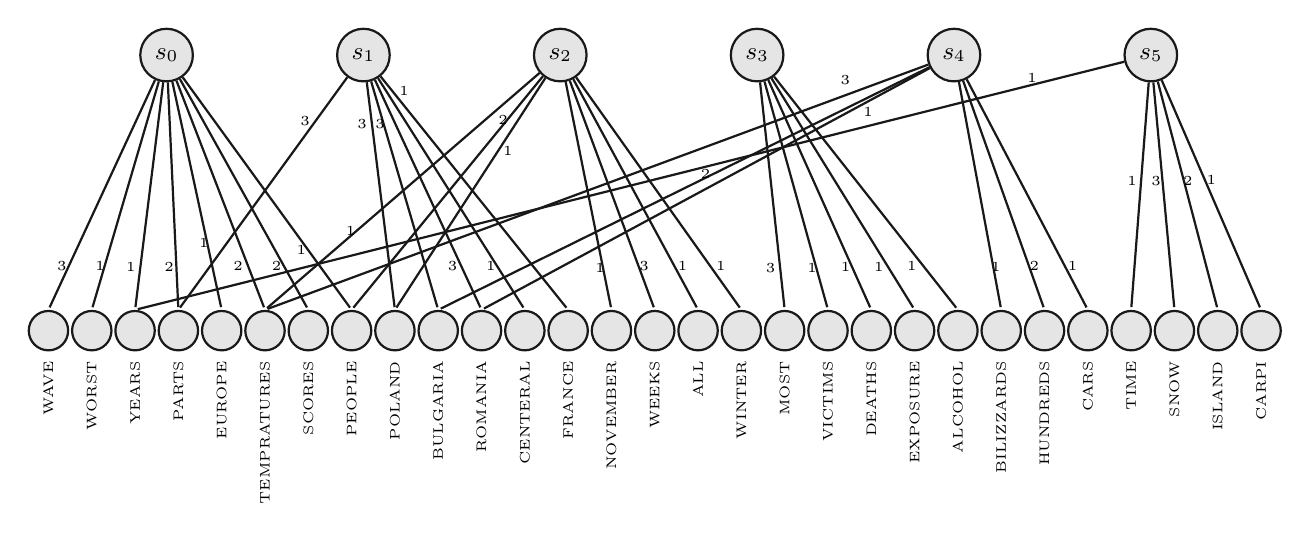
\begin{tikzpicture}[shorten >=1pt,-,scale=0.5]  
				
				\tikzstyle{sentence}=[circle,thick,draw=black!90,fill=black!10,minimum size=2mm]
				\tikzstyle{entity}=[circle,thick,draw=black!90,fill=black!10,minimum size=5mm]
				\tikzstyle{edge}=[draw=black!90, thick]
			   
			   \begin{scope}
			   
				 \node [sentence] (s0) at (-3,0) {\small{$s_0$}};
				 \node [sentence] (s1) at (2,0) {\small{$s_1$}};
				 \node [sentence] (s2) at (7,0) {\small{$s_2$}}; 
				 \node [sentence] (s3) at (12,0) {\small{$s_3$}}; 
				 \node [sentence] (s4) at (17,0) {\small{$s_4$}};
				 \node [sentence] (s5) at (22,0) {\small{$s_5$}}; 

				 \node [entity, label=below:\rotatebox{+90}{\tiny{WAVE}}] (e0)  at (-6.0,-7) {}; 
				 \node [entity, label=below:\rotatebox{+90}{\tiny{WORST}}] (e1)  at (-4.9,-7) {};
				 \node [entity, label=below:\rotatebox{+90}{\tiny{YEARS}}] (e2)  at (-3.8,-7) {}; 
				 \node [entity, label=below:\rotatebox{+90}{\tiny{PARTS}}] (e3)  at (-2.7,-7) {}; 
				 \node [entity, label=below:\rotatebox{+90}{\tiny{EUROPE}}] (e4)  at (-1.6,-7) {}; 
				 \node [entity, label=below:\rotatebox{+90}{\tiny{TEMPRATURES}}] (e5)  at (-0.5,-7) {}; 
				 \node [entity, label=below:\rotatebox{+90}{\tiny{SCORES}}] (e6)  at (0.6,-7) {}; 
				 \node [entity, label=below:\rotatebox{+90}{\tiny{PEOPLE}}] (e7)  at (1.7,-7) {}; 
				 \node [entity, label=below:\rotatebox{+90}{\tiny{POLAND}}] (e8)  at (2.8,-7) {}; 
				 \node [entity, label=below:\rotatebox{+90}{\tiny{BULGARIA}}] (e9)  at (3.9,-7) {}; 
				 \node [entity, label=below:\rotatebox{+90}{\tiny{ROMANIA}}] (e10)  at (5.0,-7) {}; 
				 \node [entity, label=below:\rotatebox{+90}{\tiny{CENTERAL}}] (e11)  at (6.1,-7) {}; 
				 \node [entity, label=below:\rotatebox{+90}{\tiny{FRANCE}}] (e12)  at (7.2,-7) {}; 
				 \node [entity, label=below:\rotatebox{+90}{\tiny{NOVEMBER}}] (e13)  at (8.3,-7) {}; 
				 \node [entity, label=below:\rotatebox{+90}{\tiny{WEEKS}}] (e14)  at (9.4,-7) {}; 
				 \node [entity, label=below:\rotatebox{+90}{\tiny{ALL}}] (e15)  at (10.5,-7) {}; 
				 \node [entity, label=below:\rotatebox{+90}{\tiny{WINTER}}] (e16)  at (11.6,-7) {}; 
				 \node [entity, label=below:\rotatebox{+90}{\tiny{MOST}}] (e17)  at (12.7,-7) {}; 
				 \node [entity, label=below:\rotatebox{+90}{\tiny{VICTIMS}}] (e18)  at (13.8,-7) {}; 
				 \node [entity, label=below:\rotatebox{+90}{\tiny{DEATHS}}] (e19)  at (14.9,-7) {}; 
				 \node [entity, label=below:\rotatebox{+90}{\tiny{EXPOSURE}}] (e20)  at (16.0,-7) {}; 
				 \node [entity, label=below:\rotatebox{+90}{\tiny{ALCOHOL}}] (e21)  at (17.1,-7) {}; 
				 \node [entity, label=below:\rotatebox{+90}{\tiny{BILIZZARDS}}] (e22)  at (18.2,-7) {}; 
				 \node [entity, label=below:\rotatebox{+90}{\tiny{HUNDREDS}}] (e23)  at (19.3,-7) {}; 
				 \node [entity, label=below:\rotatebox{+90}{\tiny{CARS}}] (e24)  at (20.4,-7) {}; 
				 \node [entity, label=below:\rotatebox{+90}{\tiny{TIME}}] (e25)  at (21.5,-7) {}; 
				 \node [entity, label=below:\rotatebox{+90}{\tiny{SNOW}}] (e26)  at (22.6,-7) {}; 
				 \node [entity, label=below:\rotatebox{+90}{\tiny{ISLAND}}] (e27)  at (23.7,-7) {}; 
				 \node [entity, label=below:\rotatebox{+90}{\tiny{CARPI}}] (e28)  at (24.8,-7) {}; 

				 
				 \path[edge] (s0) edge [above, very near end] node[font=\tiny] {$3$} (e0.north); %, line width=0.3ex
				 \path[edge] (s0) edge [above, very near end] node[font=\tiny] {$1$} (e1.north);
				 \path[edge] (s0) edge [above, very near end] node[font=\tiny, xshift=-1mm] {$1$} (e2.north);
				 \path[edge] (s0) edge [above, very near end] node[font=\tiny, xshift=-1mm] {$2$} (e3.north);
				 \path[edge] (s0) edge [above, very near end] node[font=\tiny, yshift=3mm, xshift=-1.5mm] {$1$} (e4.north);
				 \path[edge] (s0) edge [above, very near end] node[font=\tiny, xshift=-2mm] {$2$} (e5.north);
				 \path[edge] (s0) edge [above, very near end] node[font=\tiny, xshift=-2mm] {$2$} (e6.north);
				 \path[edge] (s0) edge [above, very near end] node[font=\tiny, yshift=2mm, xshift=-3.7mm] {$1$} (e7.north);

				 \path[edge] (s1) edge [above, near start] node[font=\tiny, near start] {$3$} (e3.north);
				 \path[edge] (s1) edge [above, near start] node[font=\tiny, xshift=-1.5mm] {$3$} (e8.north);
				 \path[edge] (s1) edge [above, near start] node[font=\tiny, xshift=-1mm] {$3$} (e9.north);
				 \path[edge] (s1) edge [above, very near end] node[font=\tiny, xshift=-2mm] {$3$} (e10.north);
				 \path[edge] (s1) edge [above, very near end] node[font=\tiny, xshift=-2mm] {$1$} (e11.north);
				 \path[edge] (s1) edge [above, very near start] node[font=\tiny] {$1$} (e12.north);

				 \path[edge] (s2) edge [above, very near end] node[font=\tiny, yshift=4.4mm, xshift=6.5mm] {$1$} (e5.north);
				 \path[edge] (s2) edge [above, near start] node[font=\tiny, xshift=1mm] {$2$} (e7.north);
				 \path[edge] (s2) edge [below, near start] node[font=\tiny] {$1$} (e8.north);
				 \path[edge] (s2) edge [below,  near end] node[font=\tiny] {$1$} (e13.north);
				 \path[edge] (s2) edge [above, very near end] node[font=\tiny] {$3$} (e14.north);
				 \path[edge] (s2) edge [above, very near end] node[font=\tiny] {$1$} (e15.north);
				 \path[edge] (s2) edge [above, very near end] node[font=\tiny] {$1$} (e16.north);

				 \path[edge] (s3) edge [below,  near end] node[font=\tiny,xshift=-1mm] {$3$} (e17.north);
				 \path[edge] (s3) edge [below,  near end] node[font=\tiny] {$1$} (e18.north);
				 \path[edge] (s3) edge [below,  near end] node[font=\tiny] {$1$} (e19.north);
				 \path[edge] (s3) edge [below,  near end] node[font=\tiny] {$1$} (e20.north);
				 \path[edge] (s3) edge [below,  near end] node[font=\tiny] {$1$} (e21.north);

				 \path[edge] (s4) edge [above, very near start] node[font=\tiny] {$3$} (e5.north);
				 \path[edge] (s4) edge [below, very near start] node[font=\tiny] {$1$} (e9.north);
				 \path[edge] (s4) edge [above, midway] node[font=\tiny] {$2$} (e10.north);
				 \path[edge] (s4) edge [above, very near end] node[font=\tiny] {$1$} (e22.north); 
				 \path[edge] (s4) edge [above, very near end] node[font=\tiny] {$2$} (e23.north); 
				 \path[edge] (s4) edge [above, very near end] node[font=\tiny] {$1$} (e24.north);     

				 \path[edge] (s5) edge [above, very near start] node[font=\tiny, xshift=4mm] {$1$} (e2.north);
				 \path[edge] (s5) edge [above, midway] node[font=\tiny,xshift=-1mm] {$1$} (e25.north);
				 \path[edge] (s5) edge [above, midway] node[font=\tiny,xshift=-1mm] {$3$} (e26.north);
				 \path[edge] (s5) edge [above, midway] node[font=\tiny] {$2$} (e27.north); 
				 \path[edge] (s5) edge [above, midway] node[font=\tiny] {$1$} (e28.north);   

				\end{scope}        
			  \end{tikzpicture}
		\end{tabular}
		}%
	\end{center}
	\caption{The entity graph representation of the text presented in Example \ref{ex:rel-text}. 
	The graph is obtained from the entity grid representation shown in Table \ref{tab:rel-egrid}. 
	The top nodes represent columns in the gird or sentences in the text. 
	The bottom nodes capture rows in the grid or entities in the text. 
	Edges encode the entries in the grid. 
	Weights of edges represent the value of each entry in the gird: 3:S, 2:O, 1:X, and 0:--. 
	The weight of 0 is equivalent with no edge in a graph, so they are not drawn in the graph.  
	}
	\label{fig:rel-egraph}
\end{figure}

\subsubsection{Coherence Measurement: The Average Outdegree of Projection Graphs}

\paragraph{Projection graphs.}
Local coherence is about the connectivity among sentences in a text. 
Sentences are modeled by one set of nodes in the entity graph representation, and the other set of nodes captures entities. 
\newcite{guinaudeau13} propose to transfer entity graphs to a graph whose nodes capture only sentences, and relations encode entity-based connections between sentences. 
Such a graph, which is obtained from a bipartite graph, is called a one-mode projection graph (or a projection graph for the sake of brevity) in the graph theory \cite{newmanmark10}. 
Edges in projection graphs can be weighted in different ways in order to retain specific information about  relations between sentence nodes and entity nodes in the entity graph. 
Moreover, edges in projection graphs are directed to encode the order of sentences in a text. 

\newcite{guinaudeau13} apply three kinds of projections, namely $P_U$, $P_W$ and $P_{Acc}$. 
Figure \ref{fig:rel-proj} shows these graphs obtained from the entity graph presented in Figure \ref{fig:rel-egraph}. 
These projection graphs differ in the weighting scheme that is associated with their edges: 

\begin{itemize}

	\item In $P_U$ weights are binary, i.e.\ 0 or 1. 
	The weight of an edge between two nodes in this type of the projection graph is equal to $1$ if the sentence nodes are connected to at least one entity node in the entity graph.  
	This projection graph merely captures which sentences are linked to each other in a text. 

	\item In $P_W$ an edge is weighted according to the number of the entity nodes that are connected with both sentence nodes in the entity graph. 
	In other words, the weight of an edge between two nodes in this type of the projection graph represents the number of shared entities by the corresponding sentences. 
	This projection graph not only models which sentences are connected to each other but how strongly  sentences are related. 
	It takes the number of common entities between a pair of sentences as the strength of the relation between sentences. 

	\item In $P_{Acc}$ syntactic information is accounted for by integrating the edge weights in the entity graph. 
	In this case, the weight of the edge between nodes $s_i$ and $s_k$ is equal to

	\begin{equation}
		W_{ik} = \sum_{e \in E_{ik}}{w(e,s_i) \cdot w(e,s_k)},
	\end{equation}
	%
	where $E_{ik}$ is the set of the entity nodes that are connected to both $s_i$ and $s_k$. 
	This type of the projection graph incorporates grammatical information about shared entities by sentences in order to measure the strength of the relation between sentences. 

\end{itemize}


\begin{figure}[!ht]
	\begin{center}
		\begin{tabular}{@{}lc@{}}
			\begin{tikzpicture}        
					 \node [] (n0) at (0,0) {};
			         \node [] (label) at (0,0.8) {$P_U:$};
			\end{tikzpicture}
			&
			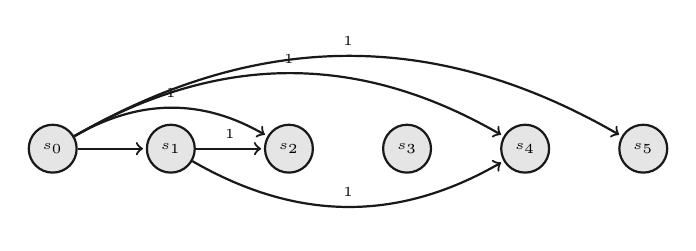
\begin{tikzpicture}[shorten >=1pt,->,scale=0.5]  
        		\tikzstyle{sentence}=[circle,thick,draw=black!90,fill=black!10,minimum size=2mm]
				\tikzstyle{entity}=[circle,thick,draw=black!90,fill=black!10,minimum size=2mm]
        		\tikzstyle{edge}=[draw=black!90, thick]

       			\begin{scope}

			         \node [sentence] (s0) at (0,0) {\tiny{$s_0$}};
			         \node [sentence] (s1) at (3,0) {\tiny{$s_1$}};
			         \node [sentence] (s2) at (6,0) {\tiny{$s_2$}}; 
			         \node [sentence] (s3) at (9,0) {\tiny{$s_3$}}; 
			         \node [sentence] (s4) at (12,0) {\tiny{$s_4$}};
			         \node [sentence] (s5) at (15,0) {\tiny{$s_5$}}; 
 
			 		\path[edge] (s0) edge [above] node[font=\tiny]{} (s1);
			 		\path[edge, bend left = 30] (s0) edge [above] node[font=\tiny]{$1$} (s2);
					\path[edge, bend left = 30] (s0) edge [above] node[font=\tiny]{$1$} (s4);
			 		\path[edge, bend left = 30] (s0) edge [above] node[font=\tiny]{$1$} (s5);

			 		\path[edge] (s1) edge [above] node[font=\tiny]{$1$} (s2);
					\path[edge, bend right = 30] (s1) edge [above] node[font=\tiny]{$1$} (s4);
           
		        \end{scope}        
     		 \end{tikzpicture}

			 \\

			\begin{tikzpicture}        
				 \node [] (n0) at (0,0) {};
        		 \node [] (label) at (0,0.8) {$P_W:$};
			\end{tikzpicture}
 			&
			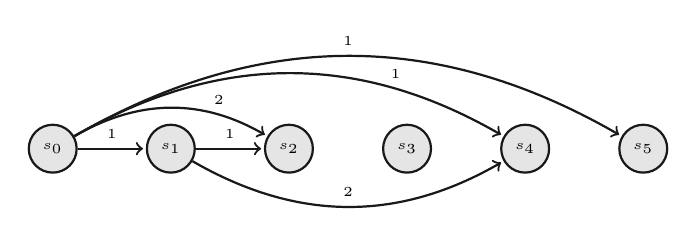
\begin{tikzpicture}[shorten >=1pt,->,scale=0.5]  
        			\tikzstyle{sentence}=[circle,thick,draw=black!90,fill=black!10,minimum size=2mm]
					\tikzstyle{entity}=[circle,thick,draw=black!90,fill=black!10,minimum size=2mm]
			        \tikzstyle{edge}=[draw=black!90, thick]
 			 
 			       \begin{scope}
       
     				    \node [sentence] (s0) at (0,0) {\tiny{$s_0$}};
				         \node [sentence] (s1) at (3,0) {\tiny{$s_1$}};
				         \node [sentence] (s2) at (6,0) {\tiny{$s_2$}}; 
				         \node [sentence] (s3) at (9,0) {\tiny{$s_3$}}; 
				         \node [sentence] (s4) at (12,0) {\tiny{$s_4$}};
				         \node [sentence] (s5) at (15,0) {\tiny{$s_5$}}; 
				 
				 		\path[edge                ] (s0) edge [above, midway] node[font=\tiny]{$1$} (s1);
				 		\path[edge, bend left = 30] (s0) edge [above, near end] node[font=\tiny]{$2$} (s2);
						\path[edge, bend left = 30] (s0) edge [above, near end] node[font=\tiny]{$1$} (s4);
				 		\path[edge, bend left = 30] (s0) edge [above, midway] node[font=\tiny]{$1$} (s5);

				 		\path[edge                 ] (s1) edge [above, midway] node[font=\tiny]{$1$} (s2);
						\path[edge, bend right = 30] (s1) edge [above, midway] node[font=\tiny]{$2$} (s4);
           
    			    \end{scope}        
   		   \end{tikzpicture}

			\\

			\begin{tikzpicture}        
				 \node [] (n0) at (0,0) {};
		         \node [] (label) at (0,0.8) {$P_{Acc}:$};
			\end{tikzpicture}
 			&

		   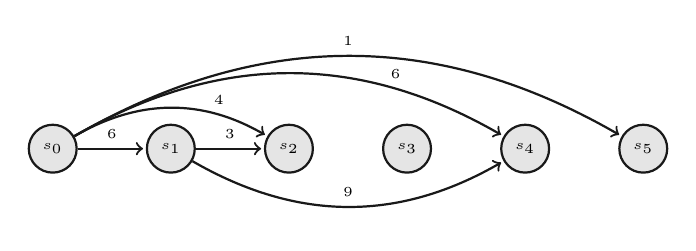
\begin{tikzpicture}[shorten >=1pt,->,scale=0.5]  
		        \tikzstyle{sentence}=[circle,thick,draw=black!90,fill=black!10,minimum size=2mm]
				\tikzstyle{entity}=[circle,thick,draw=black!90,fill=black!10,minimum size=2mm]
		        \tikzstyle{edge}=[draw=black!90, thick]

		        \begin{scope}

			         \node [sentence] (s0) at (0,0) {\tiny{$s_0$}};
			         \node [sentence] (s1) at (3,0) {\tiny{$s_1$}};
			         \node [sentence] (s2) at (6,0) {\tiny{$s_2$}}; 
			         \node [sentence] (s3) at (9,0) {\tiny{$s_3$}}; 
			         \node [sentence] (s4) at (12,0) {\tiny{$s_4$}};
			         \node [sentence] (s5) at (15,0) {\tiny{$s_5$}}; 
 
			 		\path[edge                ] (s0) edge [above, midway] node[font=\tiny]{$6$} (s1);
			 		\path[edge, bend left = 30] (s0) edge [above, near end] node[font=\tiny]{$4$} (s2);
					\path[edge, bend left = 30] (s0) edge [above, near end] node[font=\tiny]{$6$} (s4);
			 		\path[edge, bend left = 30] (s0) edge [above, midway] node[font=\tiny]{$1$} (s5);

			 		\path[edge                 ] (s1) edge [above, midway] node[font=\tiny]{$3$} (s2);
					\path[edge, bend right = 30] (s1) edge [above, midway] node[font=\tiny]{$9$} (s4);
           
		        \end{scope}        
      
      		\end{tikzpicture}

		\end{tabular}
	\end{center}
	\caption{
	Three types of projection graphs that are employed by the entity graph model. 
	$P_U$ shows only which sentence nodes are connected. 
	$P_W$ takes the number of shared entities as the weight of edges. 
	$P_{Acc}$ involves grammatical roles of common entities between sentences. 
	}
	\label{fig:rel-proj}
\end{figure}

Distances between sentences can be integrated in the weighting scheme of edges in the projection graphs to decrease the importance of links between non-adjacent sentences \cite{guinaudeau13}.   
In this case, edge weights in projection graphs are divided by the number of sentences in between of two sentences. 

\paragraph{The average outdegree as a coherence metric.}
Given a projection graph representation of a text, the coherence of the text can be measured based on the connectivity of nodes in the projection graph. 
\newcite{guinaudeau13} assume that projection graphs of coherent texts contain more edges than  projection graphs of incoherent ones.  
They propose to use a centrality metric \cite{newmanmark10} in the graph theory for measuring to what extend nodes in a projection graph are connected with each other. 
Let $outDegree(s)$ be the sum of the weights associated to edges that leave node $s$ in projection graph $P$, then the centrality metric of the projection graph is computed by the average outdegree of all nodes ($N$) in the graph: 

\begin{equation}
	 AvgOutDeg(P) = \frac{1}{N} \sum_{i=1}^{N} outDegree(s_i).
\end{equation}

Table \ref{tab:rel-od} shows the AvgOutDeg for different projection graphs presented in Figure \ref{fig:rel-proj} with and without incorporating the distance information. 

\begin{table}[!ht]
	\begin{center}
		\begin{tabular}{ll}
			\hline
			 $P$ & $ AvgOutDeg(P)$ \\\hline
			 $P_U$ & $\frac{1}{6} \left((1+1+1+1)+(1+1)+(0)+(0)+(0)+(0)) \right) = 1.00$ \\
			 $P_W$ & $\frac{1}{6} \left((1+2+1+1)+(1+2)+(0)+(0)+(0)+(0)) \right) = 1.33$\\
			 $P_{Acc}$ &$\frac{1}{6} \left((6+4+6+1)+(3+9)+(0)+(0)+(0)+(0)) \right) = 4.83$ \\
			 $P_U\textit{, }Dist$ & $\frac{1}{6} \left((1+0.50+0.25+0.20)+(1+0.33)+(0)+(0)+(0)+(0)) \right) = 0.55$ \\
			 $P_W\textit{, }Dist$ & $\frac{1}{6} \left((1+1+0.25+0.20)+(1+0.66)+(0)+(0)+(0)+(0)) \right)= 0.69$ \\
			 $P_{Acc}\textit{, }Dist$ & $\frac{1}{6} \left((6+2+1.5+0.2)+(3+3)+(0)+(0)+(0)+(0)) \right)= 2.61$ \\
			 \hline
		\end{tabular}
	\end{center}
	\caption{The average outdegree of nodes in projection graphs presented in Figure \ref{fig:rel-proj}
	. Dist.\ shows when distance is integrated in edge weights. }
	\label{tab:rel-od}
\end{table}

In order to rank a pair of texts with respect to their coherence, \newcite{guinaudeau13} represent both texts with the same type of projection graphs, and then use the average outdegree of their projection graphs to compare texts. 
It is worth to mention that the proposed entity graph model by \newcite{guinaudeau13} is an unsupervised model because the final average outdegree is directly employed for comparing two texts with respect to their coherence. 
However, average outdegree captures no information about the connectivity style of nodes in a projection graph. 
For example consider two projection graphs that are shown in Figure \ref{fig:rel-avgod-weakness}. 
These two graphs have the same average outdegree, i.e.\ five, but graph (b) is disconnected because node $s_2$ is connected to none of its preceding nodes. 
The outdegree does not capture such information about the connectivity of nodes. 

\begin{figure}[!ht]
	\begin{center}
		\begin{tabular}{@{}c@{}}
			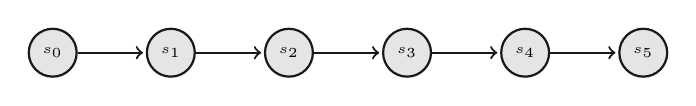
\begin{tikzpicture}[shorten >=1pt,->,scale=0.5]  
        		\tikzstyle{sentence}=[circle,thick,draw=black!90,fill=black!10,minimum size=2mm]
				\tikzstyle{entity}=[circle,thick,draw=black!90,fill=black!10,minimum size=2mm]
        		\tikzstyle{edge}=[draw=black!90, thick]

       			\begin{scope}

			         \node [sentence] (s0) at (0,0) {\tiny{$s_0$}};
			         \node [sentence] (s1) at (3,0) {\tiny{$s_1$}};
			         \node [sentence] (s2) at (6,0) {\tiny{$s_2$}}; 
			         \node [sentence] (s3) at (9,0) {\tiny{$s_3$}}; 
			         \node [sentence] (s4) at (12,0) {\tiny{$s_4$}};
			         \node [sentence] (s5) at (15,0) {\tiny{$s_5$}}; 
 
			 		\path[edge] (s0) edge (s1);
			 		\path[edge] (s1) edge (s2);
			 		\path[edge] (s2) edge (s3);
			 		\path[edge] (s3) edge (s4);
			 		\path[edge] (s4) edge (s5);
			 		
		        \end{scope}        
     		 \end{tikzpicture}
     		\\
     			(a) 
			\\
			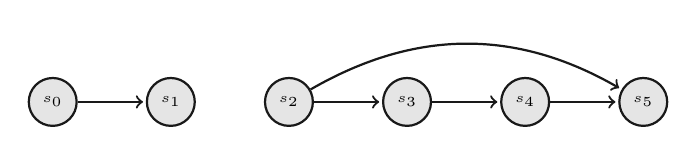
\begin{tikzpicture}[shorten >=1pt,->,scale=0.5]  
        			\tikzstyle{sentence}=[circle,thick,draw=black!90,fill=black!10,minimum size=2mm]
					\tikzstyle{entity}=[circle,thick,draw=black!90,fill=black!10,minimum size=2mm]
			        \tikzstyle{edge}=[draw=black!90, thick]
                  \begin{scope}

			         \node [sentence] (s0) at (0,0) {\tiny{$s_0$}};
			         \node [sentence] (s1) at (3,0) {\tiny{$s_1$}};
			         \node [sentence] (s2) at (6,0) {\tiny{$s_2$}}; 
			         \node [sentence] (s3) at (9,0) {\tiny{$s_3$}}; 
			         \node [sentence] (s4) at (12,0) {\tiny{$s_4$}};
			         \node [sentence] (s5) at (15,0) {\tiny{$s_5$}}; 
 
			 		\path[edge] (s0) edge (s1);
			 		
			 		\path[edge] (s2) edge (s3);
			 		\path[edge] (s3) edge (s4);
			 		\path[edge] (s4) edge (s5);
			 		\path[edge, bend left = 30] (s2) edge (s5);
                  \end{scope}
   		   \end{tikzpicture}
   		   \\
   		   (b)
   		    
		\end{tabular}
	\end{center}
	\caption{(a): A projection graph with the outdegree of five, and all nodes are in one component; (b): A projection graph with the outdegree of five with two components.}
	\label{fig:rel-avgod-weakness}
\end{figure}

Moreover, there are three types of projection graphs that behave differently in different tasks. 
So it is not clear finally which type of projection graphs should be employed for a downstream task. 

\subsubsection{Extensions of the Entity Graph Model}

The entity graph model is extended from different perspectives: text representation, and the graph metric that is employed for coherence measurement. 

\newcite{dias15} propose to fill the grid in the entity grid based on the RST relations between sentences in a text. 
An entry in the entity grid is one if an entity is part of a sentence that participate in an RST relation.
Based on such grid representation, they define a bipartite graph similar to the entity graph model, and then use the average outdegree to measure the coherence of a text. 
Their model outperforms the entity graph model. 
However, similar to RST-based extensions of the entity grid model, they argue that obtaining RST relations is subjective, and human annotation or a discourse parser is not available for many languages. 

\newcite{petersen15} use several graph metrics, rather than the average outdegree, to approximate different aspects of the text flow that can indicate coherence.  
These metrics are designed to capture more information about the connectivity style of nodes in projection graphs. 
For example, they use the mean of the PageRank scores \cite{newmanmark10}  of nodes in a projection graph to distinguish between a star-graph, in which all nodes are connected to one node and no other edges occur; and a path graph, in which all nodes occur in a chain. 
Other assessed metrics include a clustering coefficient, which measures to which extent neighbors of a node are connected among themselves; betweenness, which is the fraction of shortest paths that contain a node, and etc. 
Although their results are better than the original entity graph but the difference is not significant to use these metrics, having that the average outdegree is easy and efficient to compute. 

\newcite{zhangmuyu15} use semantic relations between named entities to not only cover 
the mentions that refer to the same entity but also the mentions that refer to entities which are semantically related (e.g.\ ``Gates'' and ``Microsoft''). 
They capture such semantic relations by leveraging WordNet \cite{baccianella10} as a knowledge base. 
They limit the semantic relation between entities to argument$_1$-predicate-argument$_2$, such as \mbox{Gates-create-Microsoft}. 
The performance of the entity graph model is improved by incorporating such relations. 
They also challenge the average outdegree metric that is used to measure the coherence of a text by the entity grid model.  
They propose to combine average outdegree with another score named reachability. 
The reachability score is the sum of the weights of edges in the shortest path that starts from the first sentence node and ends at the current sentence node. 
The intuition behind the reachability score of nodes is that this score reflects the tightness between a sentence in a text and its preceding part in the text. 
It may overcome some weaknesses of the average outdegree but not all.  

We propose\footnote{We just briefly explain this model here because it does not focus on coherence patterns which are the core of the research presented in this thesis.} \cite{mesgar14} an extension of the entity graph model by taking the entity and sentence importance into account. 
We reflect the connectivity structure of an entity graph into its edge weights by applying a normalization method to the weights.  
The normalization method reduces the differences in performance of three types of projection graphs by combining the information in these graphs. 


\section{Lexical Approaches to Local Coherence}

An important factor in text comprehension is the degree to which sentences are linked together. 
\newcite{halliday76} stressed out the role of lexical cohesion in text coherence. 
A number of linguistic devices — repetition, synonymy, hyponymy, meronymy, and etc — are considered to contribute to the ``continuity of lexical meaning'' observed in coherent text. 
In this section, we mainly survey the computational models that use lexical relations for modeling local coherence. 
However, since these models are based on the lexico-semantic relations between words in a text, we first discuss different resources that are used in the literature to recognize these relations. 

\subsection{Lexical Resources} 

Most lexical models in natural language processing, including coherence models, crucially rely on the existence of resources that encode information about semantic relations between words in a language. 
Such resources are typically acquired via two main approaches: the knowledge-based approach, or top–down, where information is manually curated by humans, and the corpus-based approach, or bottom–up, where information is automatically learned from corpora. 
Although the latter has gained ground during the last decades, due to availability of large amounts of texts and increased computing capacities, the former remains fundamental because it allows us to collect reliable, fine-grained, and explicit information. 

\paragraph{Knowledge-based resources.}
One of the fundamental lexical knowledge resources for English is the Princeton WordNet \cite{fellbaum98}.  
WordNet aims to represent real-world concepts and relations between them as they are commonly perceived by humans. 
It covers about 20 million instances extracted from row texts. 
Nouns, verbs, adjectives, and adverbs are each organized into networks of synonym sets (synsets) that each represent one underlying lexical concept and are interlinked with a variety of relations. 
WordNet-based similarity measures have been shown to correlate reliably with human similarity judgments and have been used in a variety of applications ranging from the detection of malapropisms to word sense disambiguation \cite{budanitsky06}.  
The Princeton WordNet for English inspired the creation of a lexical knowledge base in some other languages such as German, which is called GermaNet \cite{hamp97}. 
However, it is not still available for many languages because it needs human experts for annotations.  
YAGO \cite{hoffart13} is another instance of knowledge resources.  
It consists of four million instances that are automatically extracted from online encyclopedias such as WikiPedia \cite{denoyer06} and FreeBase \cite{bollacker08}. 
Relations then are edited by humans. 
Generally speaking, manually defined knowledge bases, like WordNet, have better accuracy but lower coverage, while automatically extracted knowledge bases, like YAGO, are the opposite. 

These knowledge bases are employed by different coherence models.  
\newcite{zhangmuyu15} explain two major issues for retrieving world knowledge related to words in a text: 
\begin{itemize}
\item knowledge source: Which resource is the best for obtaining this knowledge? 
\item knowledge selection: How do we pinpoint the most relevant entry in a knowledge base?
\end{itemize}
Knowledge resources cover semantic relations between certain sets of word categories.  
For example, WordNet is designed to provide complete coverage of common, open-class English words. 
Therefore, it has little or no coverage of vocabulary from specialized domains, and very limited coverage of proper nouns. 
This may hinder its application to domain-specific contexts and tasks required to deal with proper nouns. 
The issue related to knowledge selection is that if to retrieve knowledge instances using exact or partial matching. 
The chance of exact matching of words (especially entities) in a text with instances in a knowledge base is low \cite{zhangmuyu15}. 
In contrast, partial matching between arguments and entities usually increases coverage but at the risk of introducing some noise. 

In this type of knowledge resources, a simple way to compute the semantic relations between words is to view the knowledge base as a graph. 
The semantic relatedness can be measured based on graph properties such as the path length between the words \cite{budanitsky06}. 
The shorter the path between two word nodes, the more similar the words are. 

\paragraph{Corpus-based resources.} 
The bottom-up knowledge resources are obtained based on the co-occurance of words in texts in corpora. 
In these resources, words are considered similar if they occur within similar contexts. 
The semantic properties of words are captured in a multi-dimensional space by vectors that are constructed from large bodies of texts by observing the distributional patterns of co-occurrence with their neighboring words. 
The semantic relatedness between words is then measured by the similarity between their corresponding vectors. 

This type of knowledge sources differ by the method that is employed to obtain vector representations for words. 
One of the early techniques is Latent Semantic Analysis (LSA) proposed by \newcite{landauer97}. 
This method constructs a matrix, namely occurrence matrix, containing word counts per text from a large number of texts in a corpora.  
It then uses a mathematical technique called singular value decomposition (SVD) \cite{furnas88} to reduce the text dimensionality in the matrix while preserving the similarity structure among words. 

The other method is Latent Dirichlet allocation (LDA) proposed by \newcite{blei03}. 
It is a generative statistical model that allows sets of words to be explained by latent topic groups that explain why some parts of a text are similar. 
This method is identical to probabilistic latent semantic analysis (pLSA), except that in LDA the topic distribution is assumed to have a sparse Dirichlet prior.
The sparse Dirichlet priors encode the intuition that documents cover only a small set of topics and that topics use only a small set of words frequently. 
In practice, this results in a better disambiguation of words and a more precise assignment of texts to topics.
It is worth noting that in this approach a topic is neither semantically nor epistemologically strongly defined. 
It is identified on the basis of automatic detection of the likelihood of term co-occurrence. 
A lexical word may occur in several topics with a different probability, however, with a different typical set of neighboring words in each topic.

Finally, recent methods for representing words in a distributional space use deep neural networks, rather than co-occurrence matrix. 
In contrast to the primary methods that are unsupervised, the neural network models applied for obtaining word vectors are supervised.  
This property is an advantage for these methods because as the vocabulary in a language grows new vectors for new vocabulary can be trained and added to the knowledge base. 
The word vectors that are generated by these models are named word embeddings. 
Well-know approaches for obtaining word embedding are \emph{word2vec}  \cite{mikolov13} and \emph{GloVe} \cite{pennington14}. 
The word2vec approach focuses on learning the embeddings of a word given its local usage context, where the context is defined by a window of surrounding words. 
The length of the window is a configurable parameter of the model. 
Large windows tend to produce more topical similarities and smaller windows tend to produce more functional and syntactic similarities \cite{goldberg17}. 
The GloVe approach constructs an explicit word-context or word co-occurrence matrix using statistics across the whole text corpus, rather than using a window to define local context. 

Indeed, distributional representations of words, in general, are beneficial if they are trained on sufficiently large and balance corpora; otherwise there is a risk \cite{lindekang98b} of finding words which their similarity only makes sense in the corpus that is used. 
\newcite{budanitsky06} highlight more problems that arise from the imbalance and sparseness of corpora.

In this type of recourses, two words are compared by taking the cosine of the angle between their two vectors (or the dot product between the normalizations of the two vectors). 
Values close to 1 represent very semantically close words while values close to 0 represent very distant words. 

\subsection{Lexical Cohesion Models}

Here, we review local coherence models that are based on lexical relations between words. 
These relations are named lexical cohesion by \newcite{halliday76}. 
We categorize these approaches into three high-level groups: the models that are based on lexical chains, the models that are based on sentence similarities, and the probabilistic models that are based on word distributions.  

Lexical chaining has a long history in local coherence modeling for different applications \cite{morris91,fenglijun09,wongbillytm12,benguosheng13,flor13}. 
A lexical chain is a sequence of semantically related words spanning a topical text unit \cite{morris91}. 
\newcite{morris91} induce semantic relations from Roget's Thesaurus. 
The thesaurus offers a structural account of the vocabulary of English, grouping into a hierarchical  categories. 
The main intuition behind this work is that coherent texts have a high concentration of dense chains. 
Therefore, the distribution of lexical chains is a surface indicator of the structure of coherent discourse. 
\newcite{galley03a} construct lexical chains for topic segmentation, which is tightly related to coherence. 
This model does not use any knowledge resources because it builds lexical chains simply based on word repetitions. 
%They define different features of lexical chains such as length of chains. 
In contrast, \newcite{stokes04} employ WordNet to extract lexical chains from texts.  
Weak relations between words in lexical chains in a text is used as an indicator of topic shifts in the text. 
\newcite{barzilay97} propose a lexical chaining algorithm which uses WordNet, thesaurus, and POS tags to extract lexical relations. 
They do not use this model directly for coherence modeling but they utilize it for generating coherent summaries. 
\newcite{somasundaran14} use lexical chaining for measuring the quality of essays written by students. 
To do so, they employ Lin’s thesaurus \cite{lindekang98} to identify semantically similar words in essays.   
The main intuition is that the number of chains and their properties reveal the coherence of essays in terms of the focus of the topic and the elaboration of the topic. 
In order to capture different aspects of a lexical chain, they employ features of lexical chains, such as the chain size, the number of chains that contain more than one word type, and so forth. 

Another trend in research regarding local coherence modeling considers lexical relations between words of sentences in order to compute the similarity between sentences.    
The main insight is that sentences in coherent texts are semantically similar. 
So these models represent each sentence by aggregating the vectors of its words, and the similarity between two sentences is determined by the similarity of their sentence vectors. 
Specifically, the coherence of a text is measured by computing the mean of all similarities between adjacent sentences in a text. 

\begin{equation}
coh(T) = \frac{\sum_{i=0}^{N-2}sim(s_i,s_{i+1})}{N-1},
\end{equation} 
%
where $sim(s_i, s_{i+1})$ is a measure of similarity between two adjacent sentences. 
This idea is operationalized in different ways.
For example, \newcite{foltz98} employ LSA to represent each word in a sentence by a vector and then use the weighted average of word vectors to obtain sentence vectors. 
The weighting is inspired by information retrieval techniques, most notably TF-IDF, which TF stands for the \emph{Term Frequency} and IDF is the shorten of the \emph{Inverse Document Frequency}, and is performed by the log entropy transform of each word. 
The similarity between two adjacent sentences is computed by applying cosine function to sentence vectors. 
\newcite{higgins07} apply a similar strategy for essay coherence but sentences are represented by a Random Indexing (RI) model. 
\newcite{lapata05a} compute the similarity between two adjacent sentences by counting the number of exact repetitions between nouns in sentences. 
\newcite{yannakoudakis12} represent each sentence by a vector of lemmas and the Part Of Speech (POS) tags of words in sentences, and then the average of the cosine similarities between adjacent sentences encode how coherent the text is. 
%Other similar approaches are proposed by \cite{kazantseva14}. 
\newcite{hearst94, hearst97} compute the cosine similarity between adjacent windows of words, rather than adjacent sentences. 

A recent trend of research uses the probabilistic models to assign a coherence sore to a text. 
\newcite{lapata03} proposes to compute the coherence probability between two adjacent sentence based on their lexical relations. 
This probability for a given pair of sentences is obtained by a conditional probability of words in a sentence given all words of its immediately preceding sentence. 
The coherence score of a text is the product of coherence probabilities between adjacent sentences. 
Although this model does not use any external knowledge resources but it computes its own co-occurrence matrix representation of a  text, which captures how words are distributed across adjacent sentences. 
Moreover, this model is able to learn the order of word pairs, e.g.\ ``CAR'' precedes ``TIRE'' more in coherent texts or in incoherent ones.  
\newcite{lijiwei14} propose to represent words in sentences by pre-trained word embeddings. 
Then a recurrent or a recursive neural networks is used to represent each sentence based on its word embeddings. 
A window with length three is sliding through a text and for each three adjacent sentences a coherence probability is computed. 
The final coherence sore of the text is obtained by multiplying these probabilities. 

\section{Applications and Evaluations of Coherence Models}
\label{sec:rel-coh-applications}

Coherence plays a crucial role in different natural language processing applications such as automatic text summarization \cite{celikyilmaz11,linzhiheng12,fengvanessawei12a}, automatic essay scoring \cite{miltsakaki04a,higgins04,burstein10}, readability assessment \cite{pitler08,wangxinhao13}, and so forth.  
Each of these downstream tasks can be employed to evaluate a coherence model. 
In the research of this thesis, we focus on readability assessment and document summarization for evaluating our coherence model, so we review the research related to these two tasks. 
%We then briefly discuss other tasks that have been used in the literature for evaluating coherence models. 

\subsection{Readability Assessment}

Readability is a property of a text, which describes how easily the text can be read and understood.  
\newcite{dale49} define readability as 

\emph{``The sum total (including all the interactions) of all those elements within a given piece of printed material that affect the success a group of readers have with it. 
The success is the extent to which they understand it, read it at optimal speed, and find it interesting''.}

Assessing the degree of readability of a text has been a field of research for many decades. 
Early readability metrics \cite{flesch48,kincaid75} have been established as a function of shallow features of a text, such as the number of syllables per word and the number of words per sentence. 
These traditional readability metrics are still used today in many settings and domains, mainly because they are very easy and efficient to compute.  

Later research has investigated the use of statistical language models 
(uni-gram in particular) to capture the distribution of vocabulary between two readability grade levels
\cite{siluo01,collins-thompson04}. 
This is followed by an investigation on the effect of syntactic features \cite{schwarm05,heilman07,petersen09} in the assessment of text readability. 
While language model features alone outperform syntactic features in classifying texts according to their reading grade levels, the combination of these two sets of features performed the best. 

However, these features are not sufficient to encode the readability of a text  because they never go beyond the level of words and sentences. 
Indeed, a well-written text is more than a random unrelated sequence of sentences. 
In order to properly model the difficulty of a text for its readers, beside the surface features some discourse level features  are required. 
Discourse level factors (e.g. coherence) of a text play a critical role in overall understanding of the text \cite{pitler08}.  
In a coherent text, sentences are semantically related to one another so that they become less ambiguous.   
Moreover, the relation among sentences are easy to recognize and interpret for readers, and the information flows smoothly and sentence by sentence as the text progresses. 
\newcite{beigman13} use the lexical relations between words of a text to model the quality of the text. 
Their model is inspired by the fact that a text segmentation algorithm which uses information about patterns of word co-occurrences can detect sub-topic shifts in a text. 
\newcite{eisenstein08} state that coherent texts contain some proportion of more highly associated word pairs (those in subsequent sentences within the same topical unit) and of less highly associated pairs (those in sentences from different topical units).  
They illustrate the patterns of the distribution of semantically related words correlate with the writing quality. 
\newcite{pitler08} evaluate coherence features proposed by the entity grid model, and other discourse features such as the frequency of RST relations, and so on, for the readability assessment task.  

In order to investigate and compare the impacts of these features on readability assessment, two approaches are frequently employed. 
In the first approach, readability assessment is taken as a rating task \cite{pitler08,kate10}. 
Each text should be associated with a rating assigned by human judges. 
To do so, a text is judged for its readability by several human annotators each of whom assigns the text a readability rating on a n-point scale, where n is a design choice.  
The average of these ratings is taken as the final readability rating of the text. 
Now, a statistical correlation coefficient metric, e.g.\ the Pearson correlation coefficient, between values of a feature and the average human ratings of texts in a corpus is computed to measure which feature is more informative for this task. 

The second approach is to distinguish texts which are difficult to read from texts which are easy to read. 
This is mostly treated as a pairwise classification task \cite{pitler08,guinaudeau13,barzilay08}: Given a pair of texts which one is easier to read? 
In this approach all related features are taken into account to increase the predictive power of the classifier. 
However, each feature is also separately used to classify texts in order to compare a feature with the rest of features with respect to their impact on readability.  
For example, \newcite{pitler08} show that coherence features introduced by the entity grid model are the best category of features to classify texts with respect to their readability. 

\subsection{Automatic Text Summarization}

Coherence is a key factor for any automatic text generation system since the output text is supposed to be readable. 
An example of such systems is an automatic text summarization system.
The input to a summarizer is a text (or several texts in case of multi-document summarization), and the task of the system is to produce a shorter text which contains the gist of information presented in the input text(s). 
This output text, of course, should be readable and understandable to be used by humans or other NLP applications. 

The summarization task has several design choices: single- vs multi-document, and extractive vs abstractive summarization\footnote{There is another type of summarization which is called compressive summarization, where summaries are formed by compressed sentences not necessarily extracts \cite{knight00}.} \cite{hahn00}. 
Single-document summarization systems take only one input text, whereas multi-document summarizers produce a summary from a cluster of texts. 
Extractive summarizers \cite{kupiec95,carbonell98,gillick09} produce a summary by sequencing a subset of sentences from an input text; while an abstractive summarizer \cite{wanglu13b,alfonseca13} involves generating of sentences for the summary as well.   

The summarization task, in all of its variations, and coherence modeling meet in two general trends. 
The first trend, which is called summary coherence ranking \cite{barzilay08,guinaudeau13}, employs a coherence model to discriminate between pairs of summaries generated by either humans or machines. 
This trend is (almost) similar to the readability assessment task; just examined texts are summaries. 
In this trend, the performance of a coherence model is assessed by comparing rankings induced by the model against readability rankings elicited by human judges. 
A coherence model that exhibits a high agreement with human judges accurately captures the coherence properties of the machine generated texts \cite{barzilay08}. 
Although this approach can potentially be used for evaluating the quality of summaries produced by any type of summarizers but it is mainly used to compare the outputs of multi-document extractive summarization models \cite{barzilay08}. 

The second trend combines coherence metrics with automatic text summarization system with this intention to produce coherent summaries.  
This approach is more beneficial for the real application of automatic text summarization. 
For example, some papers \cite{radev04a,nenkova05} take the advantage of word repetitions in their multi-document extractive summarizers. 
Some involve assumptions about the structure of the input text to a summarizer. 
\newcite{daume02b} hypothesize a hierarchical structure (e.g.\ section, paragraph, and etc); and \newcite{teufel02} assume a flat structure for input texts. 
\newcite{teufel02} focus on summarizing the scientific articles and use lexical cohesion clues in an article for dividing it into research goal (aim), outline of the paper (textual), presentation of the paper's contribution (methods, results, and discussion), and presentation of other work (other). 
These segments are not necessarily consistent with the physical structure of an article and can be evenly distributed through the whole article. 
This strategy is especially fruitful if a summary should contain information about specific parts of a text rather than on the text as a whole.  
\newcite{barzilay97} employ lexical chains occurring in a text to divide the text into some segments.  
The use of lexical chains allows topicality to be taken into account to heighten the quality of summaries.
\newcite{celikyilmaz10,celikyilmaz11} incorporate the idea of hierarchical topical coherence models for segmentation and sentence extraction. 
\newcite{clarke10} require the entity that serves as the center of a sentence (in the sense of the centering theory) be retained in a summary. 
\newcite{mckeown99} present a \mbox{two-stage} system in which sentences are initially clustered, and then representative sentences are chosen from each cluster to be included into the final summary. 
Here, the clustering stage minimizes redundancy and the representative sentence selection maximizes importance.
\newcite{jha15} consider Minimum Independent Discourse Contexts (MIDC) to solve the problem of non-coherence in extractive summarization.
However, this model does not deal with the problem of coherence within the task of sentence selection. 
\newcite{carbonell98} propose a global model through the use of the Maximum Marginal Relevance (MMR) criteria, which scores sentences under consideration as a weighted combination of importance plus redundancy with sentences already in the summary. 
Summaries are then created with an approximate greedy procedure that incrementally includes the sentence that maximizes this criteria. Greedy MMR style algorithms are still a standard baseline for summarization. 

One of the popular approaches for optimizing three major factors for summarization -- importance, variance and coherence -- is the Integer Linear Programming (ILP) formulation. 
ILP techniques have been used to solve many intractable inference problems in NLP applications. 
Examples include applications to sentence compression \cite{clarke10,filippova13}, coreference resolution \cite{denis09},  syntactic parsing \cite{klenner07a}, as well as semantic role labeling \cite{punyakanok04b}.
%\cite{marciniak05b,mcdonald07,bergkirkpatrick11,woodsend12,lichen13a,hirao13}.
In an ILP approach, an optimization problem is modeled by an objective function and some constraints. 
Solving arbitrary ILPs is an \mbox{NP-hard} problem. 
However, ILPs are a well studied optimization problem with efficient \mbox{branch-and-bound} algorithms for finding the optimal solution. 
Similar to the other NLP applications, ILP has been popularly employed for automatic summarization 
\cite{nishikawa10,galanis12,marciniak05b,mcdonald07,bergkirkpatrick11,woodsend12,lichen13a,hirao13}.  

\newcite{parveen15a} propose an automatic summarizer using ILP.  
The objective of the optimization is to select a subset of sentences from an input document such that the selected sentences produce a summary that is optimal in terms of importance, non-redundancy, and coherence. 
This model is of our interest because it sets up the optimization problem on the entity graph representations of texts. 
Given an input text, the importance and non-redundancy of selected sentences for a summary are measured by the bipartite entity graph of the input text. 
They employ entities as the unit of information that relate sentences because they can also be employed to measure the importance, diversity of sentences in a summary. 
Sentences that contain prominent entities of a text are important to be extracted. 
A summary whose sentences refer to few entities may contain redundant information. 
The order of sentences in a summary and the way that they share entities make the summary coherent. 
They use the outdegree of each node in the projection graph of the input text to measure how crucial the corresponding sentence with the node is for coherence of the summary.  
In Chapter \ref{ch:coh-patterns}, we employ this model to evaluate our coherence patterns by involving them into a summarizer instead of the outdegree feature in this model. 

